\documentclass[a4paper,12pt]{article}
\usepackage{fontspec,xeCJK,geometry,graphicx,booktabs,hyperref}
\IfFontExistsTF{Noto Serif CJK SC}{\setCJKmainfont{Noto Serif CJK SC}}{\setCJKmainfont{Songti SC}}
\geometry{left=1in,right=1in,top=1in,bottom=1in}
\hypersetup{hidelinks}
\begin{document}
\begin{titlepage}
\centering \vspace*{2cm}
{\Huge\bfseries 深 圳 大 学 实 验 报 告\par}
\vspace{1.5cm}
{\Large 课程名称：Python程序设计\par}
\vspace{0.5cm}
{\Large 项目名称：基于 NumPy 的图像特征提取\par}
\vspace{0.5cm}
{\Large 学院：人工智能学院\par}
\vspace{0.5cm}
{\Large 专业：\underline{\hspace{5cm}}\par}
\vspace{0.5cm}
{\Large 指导教师：舒婷\par}
\vspace{0.5cm}
{\Large 报告人：\underline{\hspace{3cm}}\quad 学号：\underline{\hspace{3cm}}\par}
\vspace{0.5cm}
{\Large 实验时间：2026年11月\par}
\vspace{0.5cm}
{\Large 提交时间：\underline{\hspace{5cm}}\par}
\vfill {\Large 教务处制\par}
\end{titlepage}

\section{Objectives：任务}
本项目在给定 OpenCLIP ViT-B/32 图像权重的条件下，使用 NumPy 实现图像编码器前向计算，不进行模型训练。输入为预处理后的 float32 图像批次 $[B,3,224,224]$；输出为每张图像一个单位长度的 512 维特征 $[B,512]$。独立提供的阶段结果用于验证数值正确性。

\section{Overview：方法与数据流程}
提供的预处理模块完成缩放、中心裁剪和通道归一化。每张图像切成 $7\times7$ 个 $32\times32$ 图像块，每块按通道、高、宽顺序展平为 3072 个值，投影至 768 维。前置 CLS token 并加入位置向量后，经过前置归一化和 12 个 Transformer 块；取最终 CLS token，经过后置归一化、投影和长度归一化，得到最终特征。固定权重只用于前向计算；参考数组只用于检查。

\begin{figure}[h]
\centering
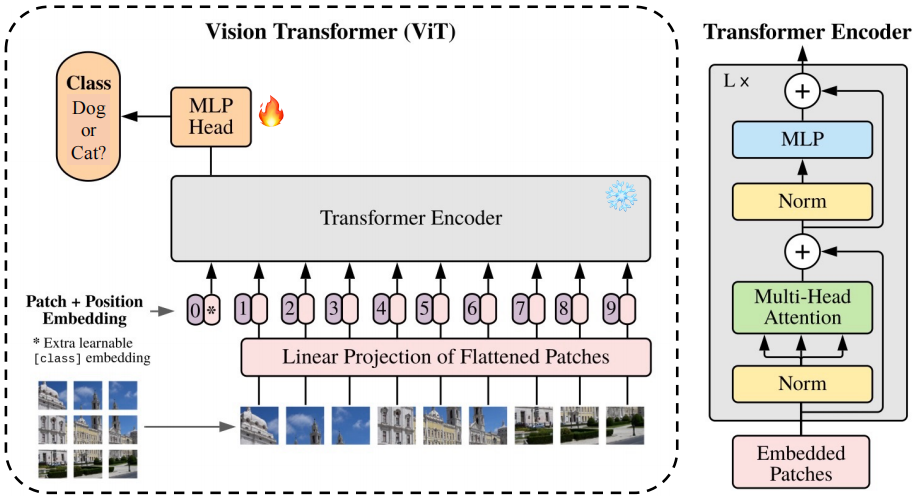
\includegraphics[width=0.68\linewidth]{figs/vit_overview.png}
\caption{ViT 图像编码流程（课程模板提供）}
\end{figure}

\section{Implementations：关键实现与贡献}
\textbf{图像块和嵌入。} \texttt{patchify} 先将输入重排为 $[B,3,7,32,7,32]$，再交换网格轴与通道轴，得到 $[B,7,7,3,32,32]$，最后展平为 $[B,49,3072]$。投影后拼接 CLS 和位置向量，得到 $[B,50,768]$。轴顺序决定每块的像素排列。

\textbf{注意力和 Transformer。} 每个 768 维 token 分成 12 个 64 维头。查询与键相乘并除以 $\sqrt{64}$，经 softmax 加权值向量；合并 12 个头并投影。每块包含注意力残差与 MLP 残差，MLP 使用给定的精确 GELU。最终选择 CLS，乘形状为 $[768,512]$ 的投影矩阵，并缩放成单位向量。

\textbf{贡献与辅助。} 六组练习的 NumPy 实现、项目说明和本报告草稿由 Codex 辅助生成。提交者需逐段检查代码与报告，并补充本人实际完成的修改、调试和验证记录。提供的预处理、辅助函数、权重、样例图像和参考检查器不计作本人原创实现。

\section{Results：结果与证据}
运行环境为 Python 3.14.3、NumPy 2.4.4、Pillow 12.2.0。运行 \texttt{python3 check.py --stage all}，全部阶段通过。各阶段与独立 FP32 参考的绝对误差如下：

\begin{center}
\small
\begin{tabular}{lccc}
\toprule
阶段 & 输出形状 & 最大绝对误差 & 平均绝对误差 \\
\midrule
预处理 & $(10,3,224,224)$ & $0$ & $0$ \\
图像块 & $(2,49,3072)$ & $0$ & $0$ \\
输入 token & $(2,50,768)$ & $0$ & $0$ \\
首个块 & $(2,50,768)$ & $7.540\times10^{-6}$ & $2.274\times10^{-7}$ \\
最后 token & $(2,50,768)$ & $4.387\times10^{-5}$ & $2.406\times10^{-6}$ \\
最终输出 & $(10,512)$ & $6.780\times10^{-7}$ & $8.215\times10^{-8}$ \\
变序及重复批次 & $(3,512)$ & $4.619\times10^{-7}$ & $8.133\times10^{-8}$ \\
\bottomrule
\end{tabular}
\end{center}
最终输出容差为 $\mathrm{atol}=2\times10^{-5},\mathrm{rtol}=2\times10^{-4}$；内部 token 容差为 $\mathrm{atol}=2\times10^{-4},\mathrm{rtol}=2\times10^{-4}$。所有结果均为有限的 float32 数值。项目 GitHub 地址：\url{https://github.com/xiaogex57/project1-numpy-image-encoder}。

\section{Discussion：分析与反思}
图像块和输入 token 的误差为零，说明轴重排、patch 投影和位置顺序与参考一致。经过 12 个块后内部 token 最大误差为 $4.387\times10^{-5}$，仍在容差内；最终输出最大误差为 $6.780\times10^{-7}$。改变批次顺序并重复图像仍通过，支持按输入行独立处理的结论。

原始项目首次运行检查时，\texttt{patches} 阶段因 TODO-01 抛出 \texttt{NotImplementedError}；补全图像块排列后该阶段误差降为零。实现中还需注意两种权重方向：大多数线性层权重是 $[\mathrm{out},\mathrm{in}]$，计算时转置；最终 \texttt{visual.proj} 已是 $[768,512]$，不转置。多头键矩阵也只交换最后两个轴。实验仅验证固定权重的前向数值一致性，不评价分类准确率或训练效果。

\newpage
\noindent\textbf{指导教师批阅意见：}
\vspace{6cm}

\noindent\textbf{成绩评定：}
\vspace{3cm}

\noindent\hfill\textbf{指导教师签字：}\quad\quad\quad\quad\quad\\[0.5cm]
\hfill\textbf{年}\quad\textbf{月}\quad\textbf{日}

\vfill
\noindent\textbf{备注：}报告内的项目或内容设置，可根据实际情况加以调整和补充。
\end{document}
